\documentclass[final]{beamer}

\usepackage{tikz}

\usepackage[scale=1.24]{beamerposter} % Use the beamerposter package for laying out the poster

\usetheme{confposter} % Use the confposter theme supplied with this template

\setbeamercolor{block title}{fg=isured,bg=white} % Colors of the block titles
\setbeamercolor{block body}{fg=black,bg=white} % Colors of the body of blocks
\setbeamercolor{block alerted title}{fg=white,bg=isugold} % Colors of the highlighted block titles
\setbeamercolor{block alerted body}{fg=black,bg=white} % Colors of the body of highlighted blocks
% Many more colors are available for use in beamerthemeconfposter.sty

%-----------------------------------------------------------
% Define the column widths and overall poster size
% To set effective sepwid, onecolwid and twocolwid values, first choose how many columns you want and how much separation you want between columns
% In this template, the separation width chosen is 0.024 of the paper width and a 4-column layout
% onecolwid should therefore be (1-(# of columns+1)*sepwid)/# of columns e.g. (1-(4+1)*0.024)/4 = 0.22
% Set twocolwid to be (2*onecolwid)+sepwid = 0.464
% Set threecolwid to be (3*onecolwid)+2*sepwid = 0.708

\newlength{\sepwid}
\newlength{\onecolwid}
\newlength{\twocolwid}
\newlength{\threecolwid}
\setlength{\paperwidth}{48in} % A0 width: 46.8in
\setlength{\paperheight}{36in} % A0 height: 33.1in
\setlength{\sepwid}{0.024\paperwidth} % Separation width (white space) between columns
\setlength{\onecolwid}{0.22\paperwidth} % Width of one column
\setlength{\twocolwid}{0.464\paperwidth} % Width of two columns
\setlength{\threecolwid}{0.708\paperwidth} % Width of three columns
\setlength{\topmargin}{-0.5in} % Reduce the top margin size
%-----------------------------------------------------------

\usepackage{graphicx}  % Required for including images

\usepackage{booktabs} % Top and bottom rules for tables

%----------------------------------------------------------------------------------------
%	TITLE SECTION 
%----------------------------------------------------------------------------------------

\title{Bayesian Functional Data Analysis and Influenza} % Poster title

\author{Nehemias Ulloa, Jarad Niemi} % Author(s)

\institute{Iowa State Univeristy} % Institution(s)



%----------------------------------------------------------------------------------------

\begin{document}

\addtobeamertemplate{headline}{} 
{\begin{tikzpicture}[remember picture, overlay]
     \node [anchor=north east, inner sep=3cm]  at (current page.north east)
     {
\includegraphics[height=4cm]{plots/isu-color-stacked.jpg}};
  \end{tikzpicture}}

\addtobeamertemplate{block end}{}{\vspace*{2ex}} % White space under blocks
\addtobeamertemplate{block alerted end}{}{\vspace*{2ex}} % White space under highlighted (alert) blocks

\setlength{\belowcaptionskip}{2ex} % White space under figures
\setlength\belowdisplayshortskip{2ex} % White space under equations

\begin{frame}[t] % The whole poster is enclosed in one beamer frame

\begin{columns}[t] % The whole poster consists of three major columns, the second of which is split into two columns twice - the [t] option aligns each column's content to the top

\begin{column}{\sepwid}\end{column} % Empty spacer column

\begin{column}{\onecolwid} % The first column

%----------------------------------------------------------------------------------------
%	OBJECTIVES
%----------------------------------------------------------------------------------------

\begin{alertblock}{ILINet}

\begin{itemize}
\item U.S. Outpatient Influenza-like Illness Surveillance Network (ILINet) via Centers for Disease Control and Prevention (CDC)
\item ILINet consists of over 3,500 enrolled outpatient healthcare providers %approx 2000 turn in numbers
\begin{itemize}
\item Total number of patients seen for any reason 
\item Number of those patients with influenza-like illness (ILI) by age group 
%(0-4 years, 5-24 years, 25-49 years, 50-64 years, and ≥65 years)
\end{itemize}
\end{itemize}

\end{alertblock}

%----------------------------------------------------------------------------------------
%	QUICK REVISION
%----------------------------------------------------------------------------------------

\begin{block}{Functional Data Analysis}

\begin{itemize}
\item Consider the entire season (function) as a data point
\item Think of weekly observation as discrete observations of a smooth underlying process
\end{itemize}
\end{block}

\begin{block}{Data + Model}

\begin{itemize}
\item $y_{r,s}(w)$ - proportion of patients with Influenza-like illness in week $w$, region $r$, season $s$
\item $\hat{\mu}(w)$ - estimated weekly means across regions and seasons
\item $\theta_{r,s}(w)$ - smooth underlying function of $w$ in region $r$, season $s$
\item $\epsilon_{r,s}(w)$ - observational error
\end{itemize}

A functional data model can be written as such:

\begin{align}
y_{r,s}(w) - \hat{\mu}(w) &= \theta_{r,s}(w) + \epsilon_{r,s}(w) \\
\epsilon_{r,s}(w) &\overset{ind}{\sim} N(0,\sigma^2_{\epsilon}) \nonumber
\end{align}

\vspace{10mm}

\textbf{Basis Choices} \\

Possible basis are: \\

\begin{itemize}
\item Polynomial bases
\item Fourier basis
\item Principal componant basis \\
\end{itemize}

\vspace{10mm}

\textbf{Functional Principled Component Analysis} \\

The FPCA method (Dauxois and Pousse (1976)) is represented like this:
\begin{equation}
  \theta_{r,s} (w) = \sum_{k=1}^{K} \beta_{r,s,k} \phi_k (w)
\end{equation}



\textbf{15-16 Influenza Season}

\end{block}

%------------------------------------------------

\begin{figure}
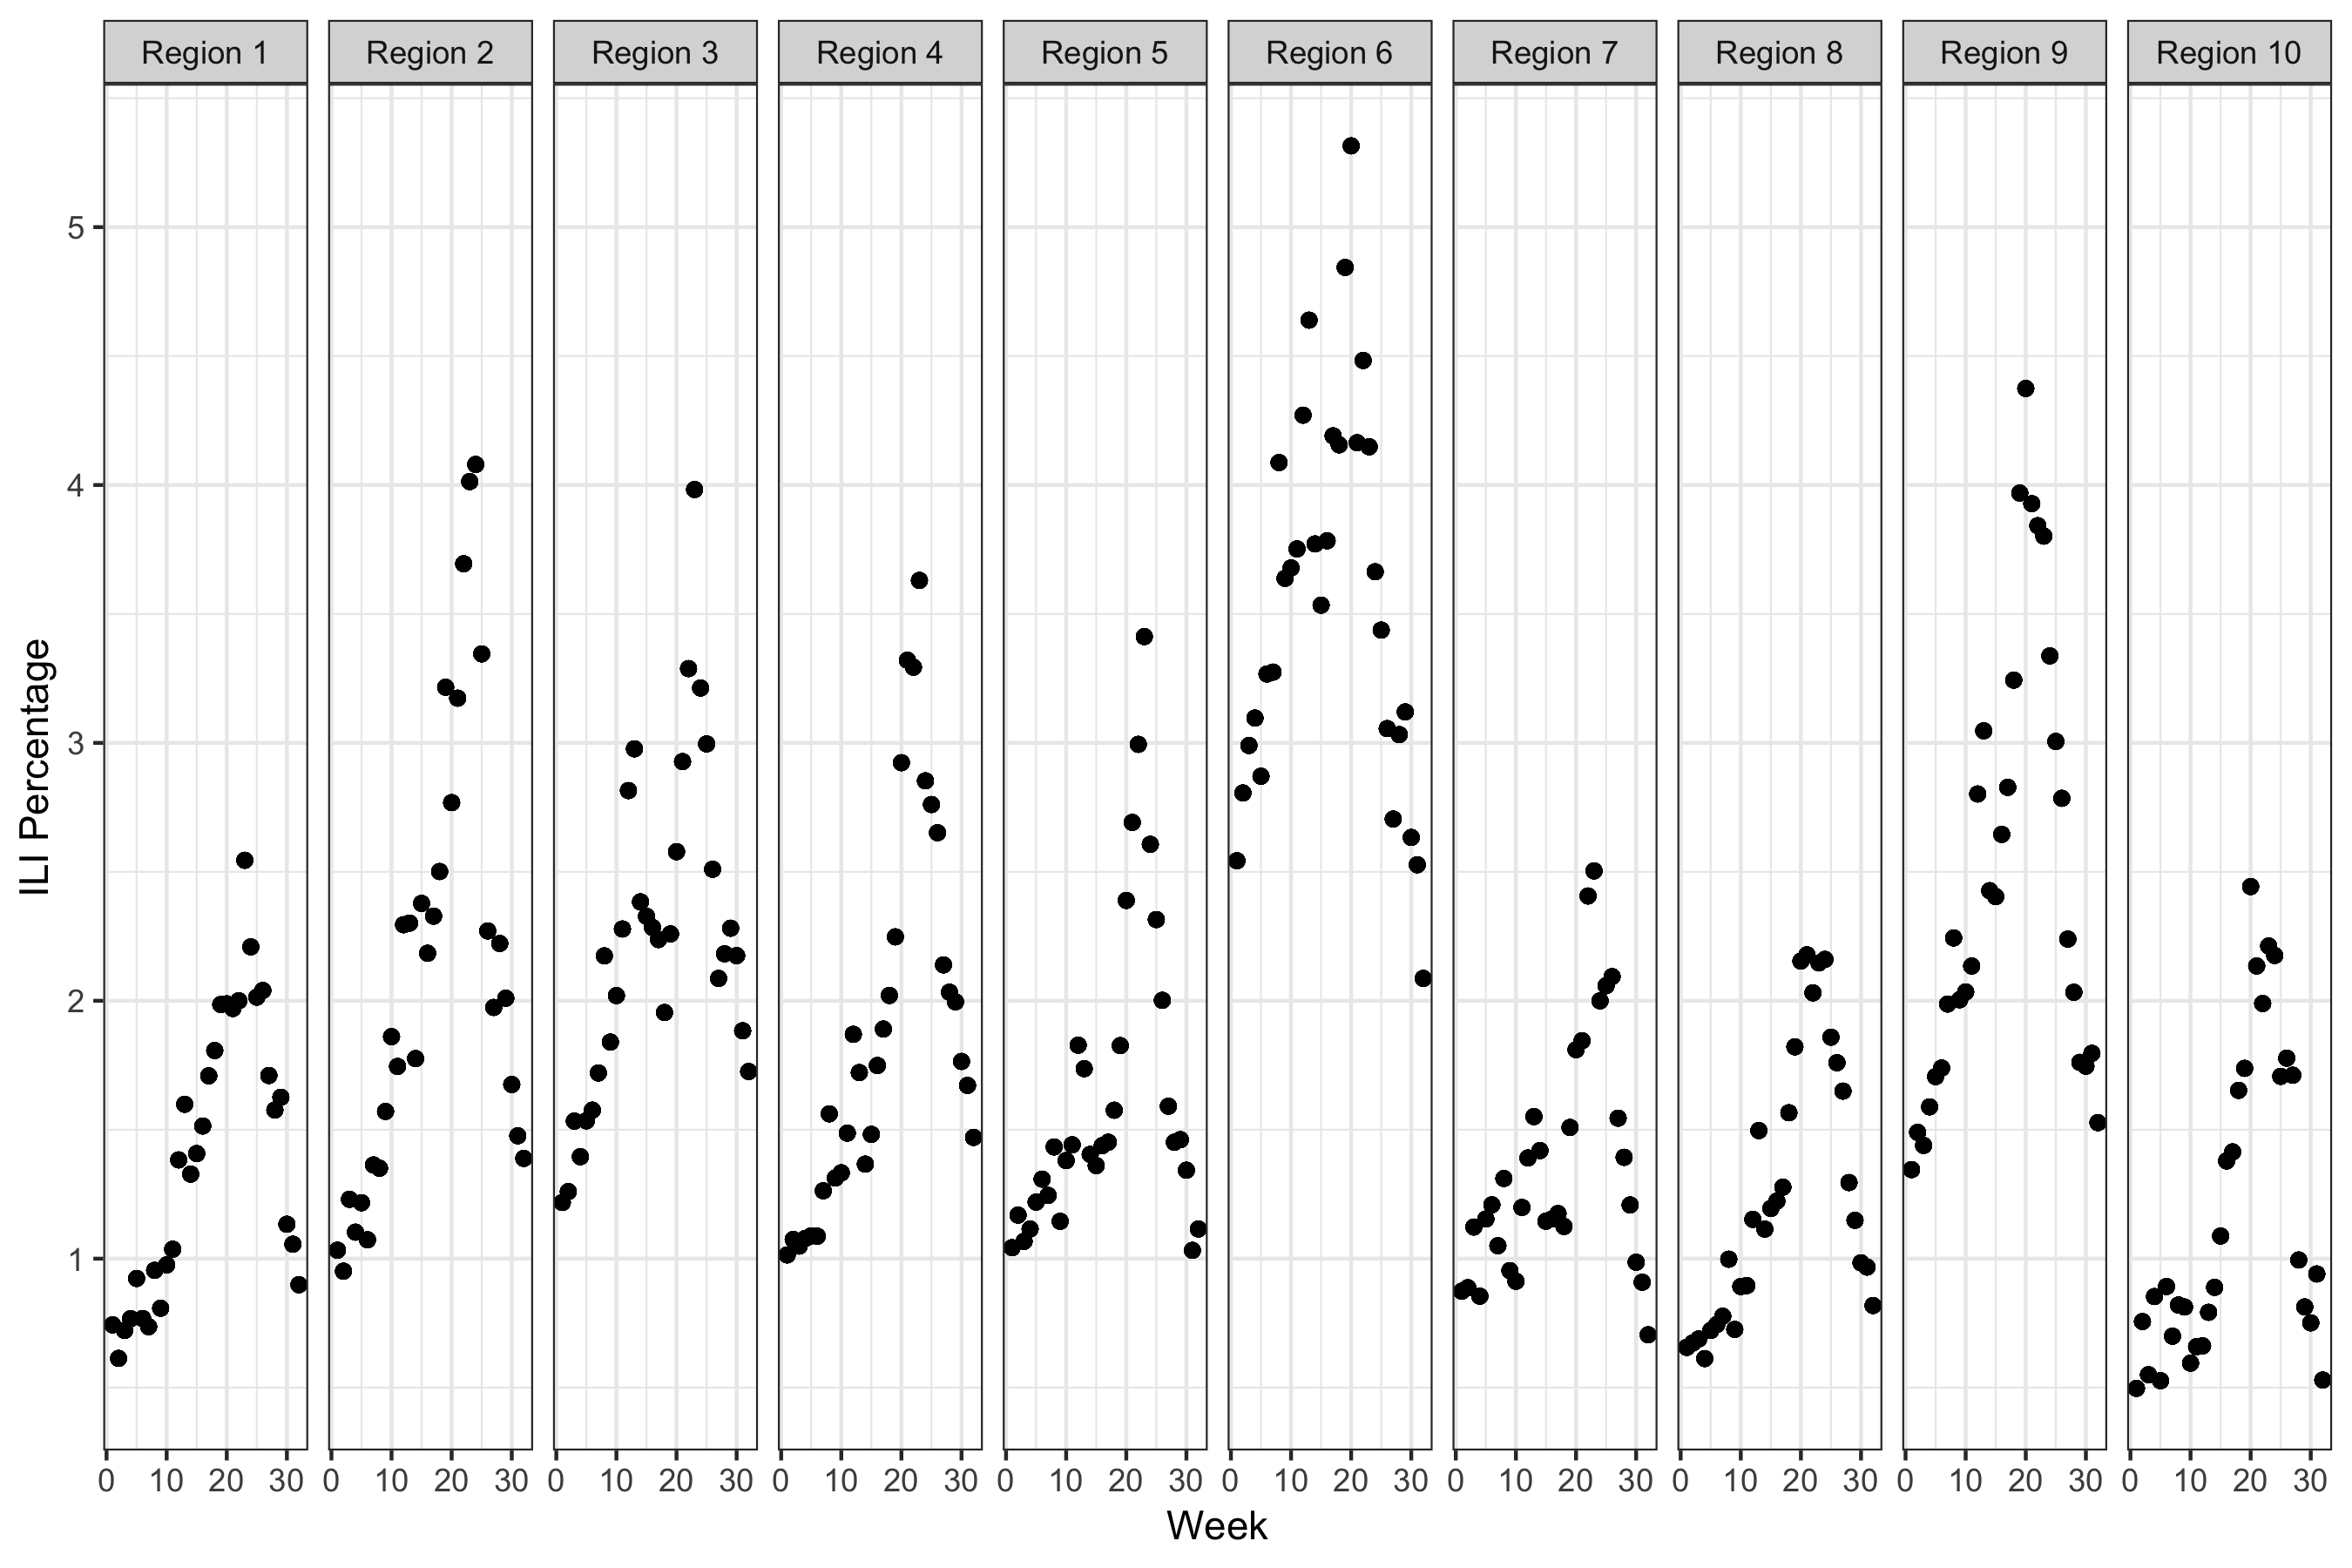
\includegraphics[width=\linewidth]{plots/ILI.png}
\caption{The 2015-2016 influenza season faceted by region.}
\end{figure}

%----------------------------------------------------------------------------------------

\end{column} % End of the first column

\begin{column}{\sepwid}\end{column} % Empty spacer column

\begin{column}{\twocolwid} % Begin a column which is two columns wide (column 2)

\begin{columns}[t,totalwidth=\twocolwid] % Split up the two columns wide column

\begin{column}{\onecolwid}\vspace{-.6in} % The first column within column 2 (column 2.1)

%----------------------------------------------------------------------------------------
%	MATERIALS
%----------------------------------------------------------------------------------------

\begin{block}{Sparse Priors for Basis Selection}

Wang et al, (2015):
\begin{itemize}
\item Point out the question of how large should $K$ be?
\item Amount of variance is accounted for and the arbitrary cutoff value is chosen
\item AIC and BIC as well as Leave one out Cross Validation (LOO CV) but they include too many components \\
\end{itemize}

\vspace{10mm}

\textbf{Horseshoe Prior}

The horseshoe prior (Carvalho et al. (2009)) model is noted by:
\begin{align}
y &\sim N(X\beta, \sigma^2 I) \nonumber \\
\beta_{r,s,i} &\overset{ind}{\sim} \text{HS}(\tau_{r,s})
\end{align}

where $\text{HS}$ is a scale mixture of normals:
\begin{align}
\beta_{r,s,i} | \lambda_{r,s}, \tau_{r,s} &\sim N(0, \lambda_{r,s,i}^2 \tau_{r,s}^2) \nonumber \\
\lambda_{r,s,i} &\overset{ind}{\sim} Ca^{+}(0,1)
\end{align}

\end{block}

%----------------------------------------------------------------------------------------

\end{column} % End of column 2.1

\begin{column}{\onecolwid}\vspace{-.6in} % The second column within column 2 (column 2.2)

%----------------------------------------------------------------------------------------
%	P
%----------------------------------------------------------------------------------------

\begin{block}{Sparse Priors for Basis Selection (cont'd)}
\textbf{Hierarchical Prior}

The hierarchical prior (Piironen and Vehtari (2017)) is similar to the horseshoe but has a half-t prior:
\begin{align}
y &\sim N(X\beta, \sigma^2 I) \nonumber \\
\beta_{r,s,i} | \lambda_{r,s}, \tau_{r,s} &\sim N(0, \lambda_{r,s,i}^2 \tau_{r,s}^2) \nonumber \\
\lambda_{r,s,i} &\overset{ind}{\sim} t^{+}_{4}(0,1)
\end{align}

\vspace{10mm}

\textbf{LASSO Prior}

The LASSO prior (Park and Casella (2008)) is a simpler shrinkage prior that the horseshoe type priors:
\begin{align}
y &\sim N(X\beta, \sigma^2 I) \nonumber \\
\beta_{r,s,i} | \lambda_{r,s}, \tau_{r,s} &\sim N(0, \lambda_{r,s,i}^2) \nonumber \\
\lambda_{r,s,i} &\overset{ind}{\sim} Laplace(a,b)
\end{align}

\end{block}

%----------------------------------------------------------------------------------------

\end{column} % End of column 2.2

\end{columns} % End of the split of column 2 - any content after this will now take up 2 columns width

%----------------------------------------------------------------------------------------
%	IMPORTANT To REMEMBER
%----------------------------------------------------------------------------------------

\begin{alertblock}{Questions of Interest}

\begin{itemize}
  \item Does these methods work to model the influenza season?
  \item Do the shrinkage priors naturally choose the number of basis functions?
  \item Can it forecast a new season?
\end{itemize}

\end{alertblock} 

\begin{block}{Model Fit}
\begin{figure}
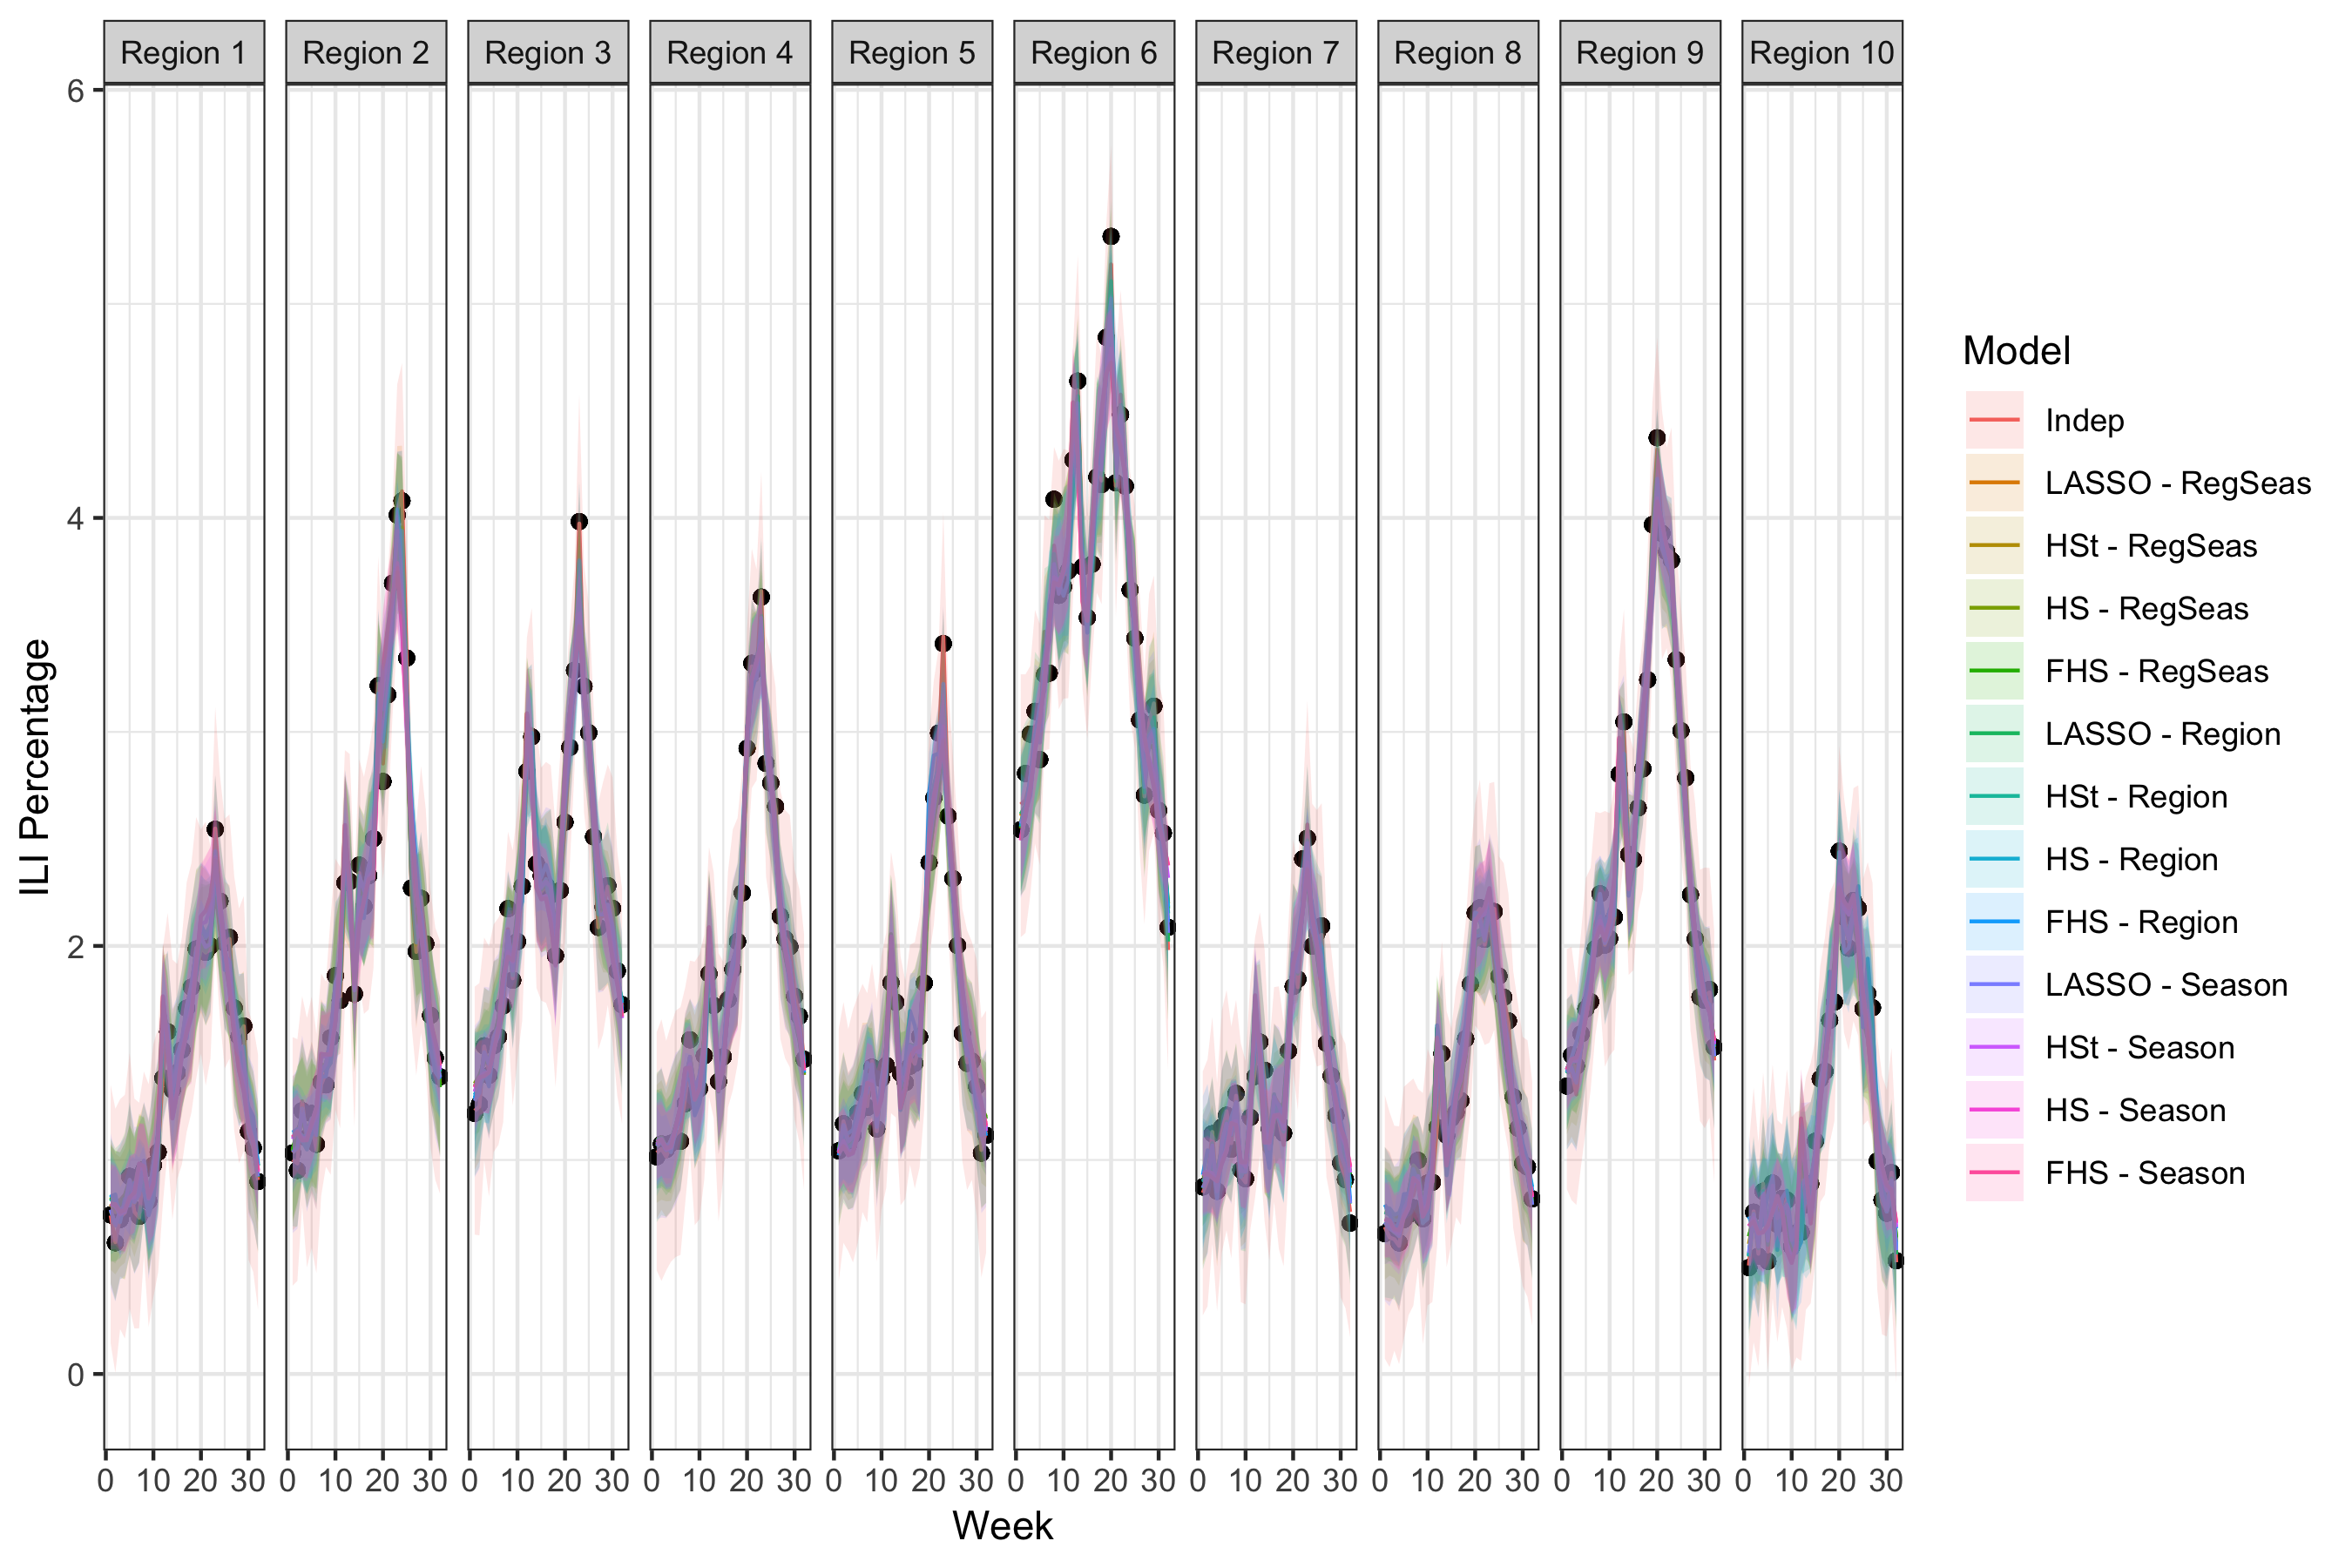
\includegraphics[width=\linewidth]{plots/ILIfit.png}
\caption{The 2015-2016 influenza season faceted by region.}
\end{figure}
\end{block}

%----------------------------------------------------------------------------------------

\begin{columns}[t,totalwidth=\twocolwid] % Split up the two columns wide column again

\begin{column}{\onecolwid} % The first column within column 2 (column 2.1)

%----------------------------------------------------------------------------------------
%	EXAMPLE OF FACTORISATION
%----------------------------------------------------------------------------------------

% \begin{block}{Model Fit}
% 
% \begin{figure}
% 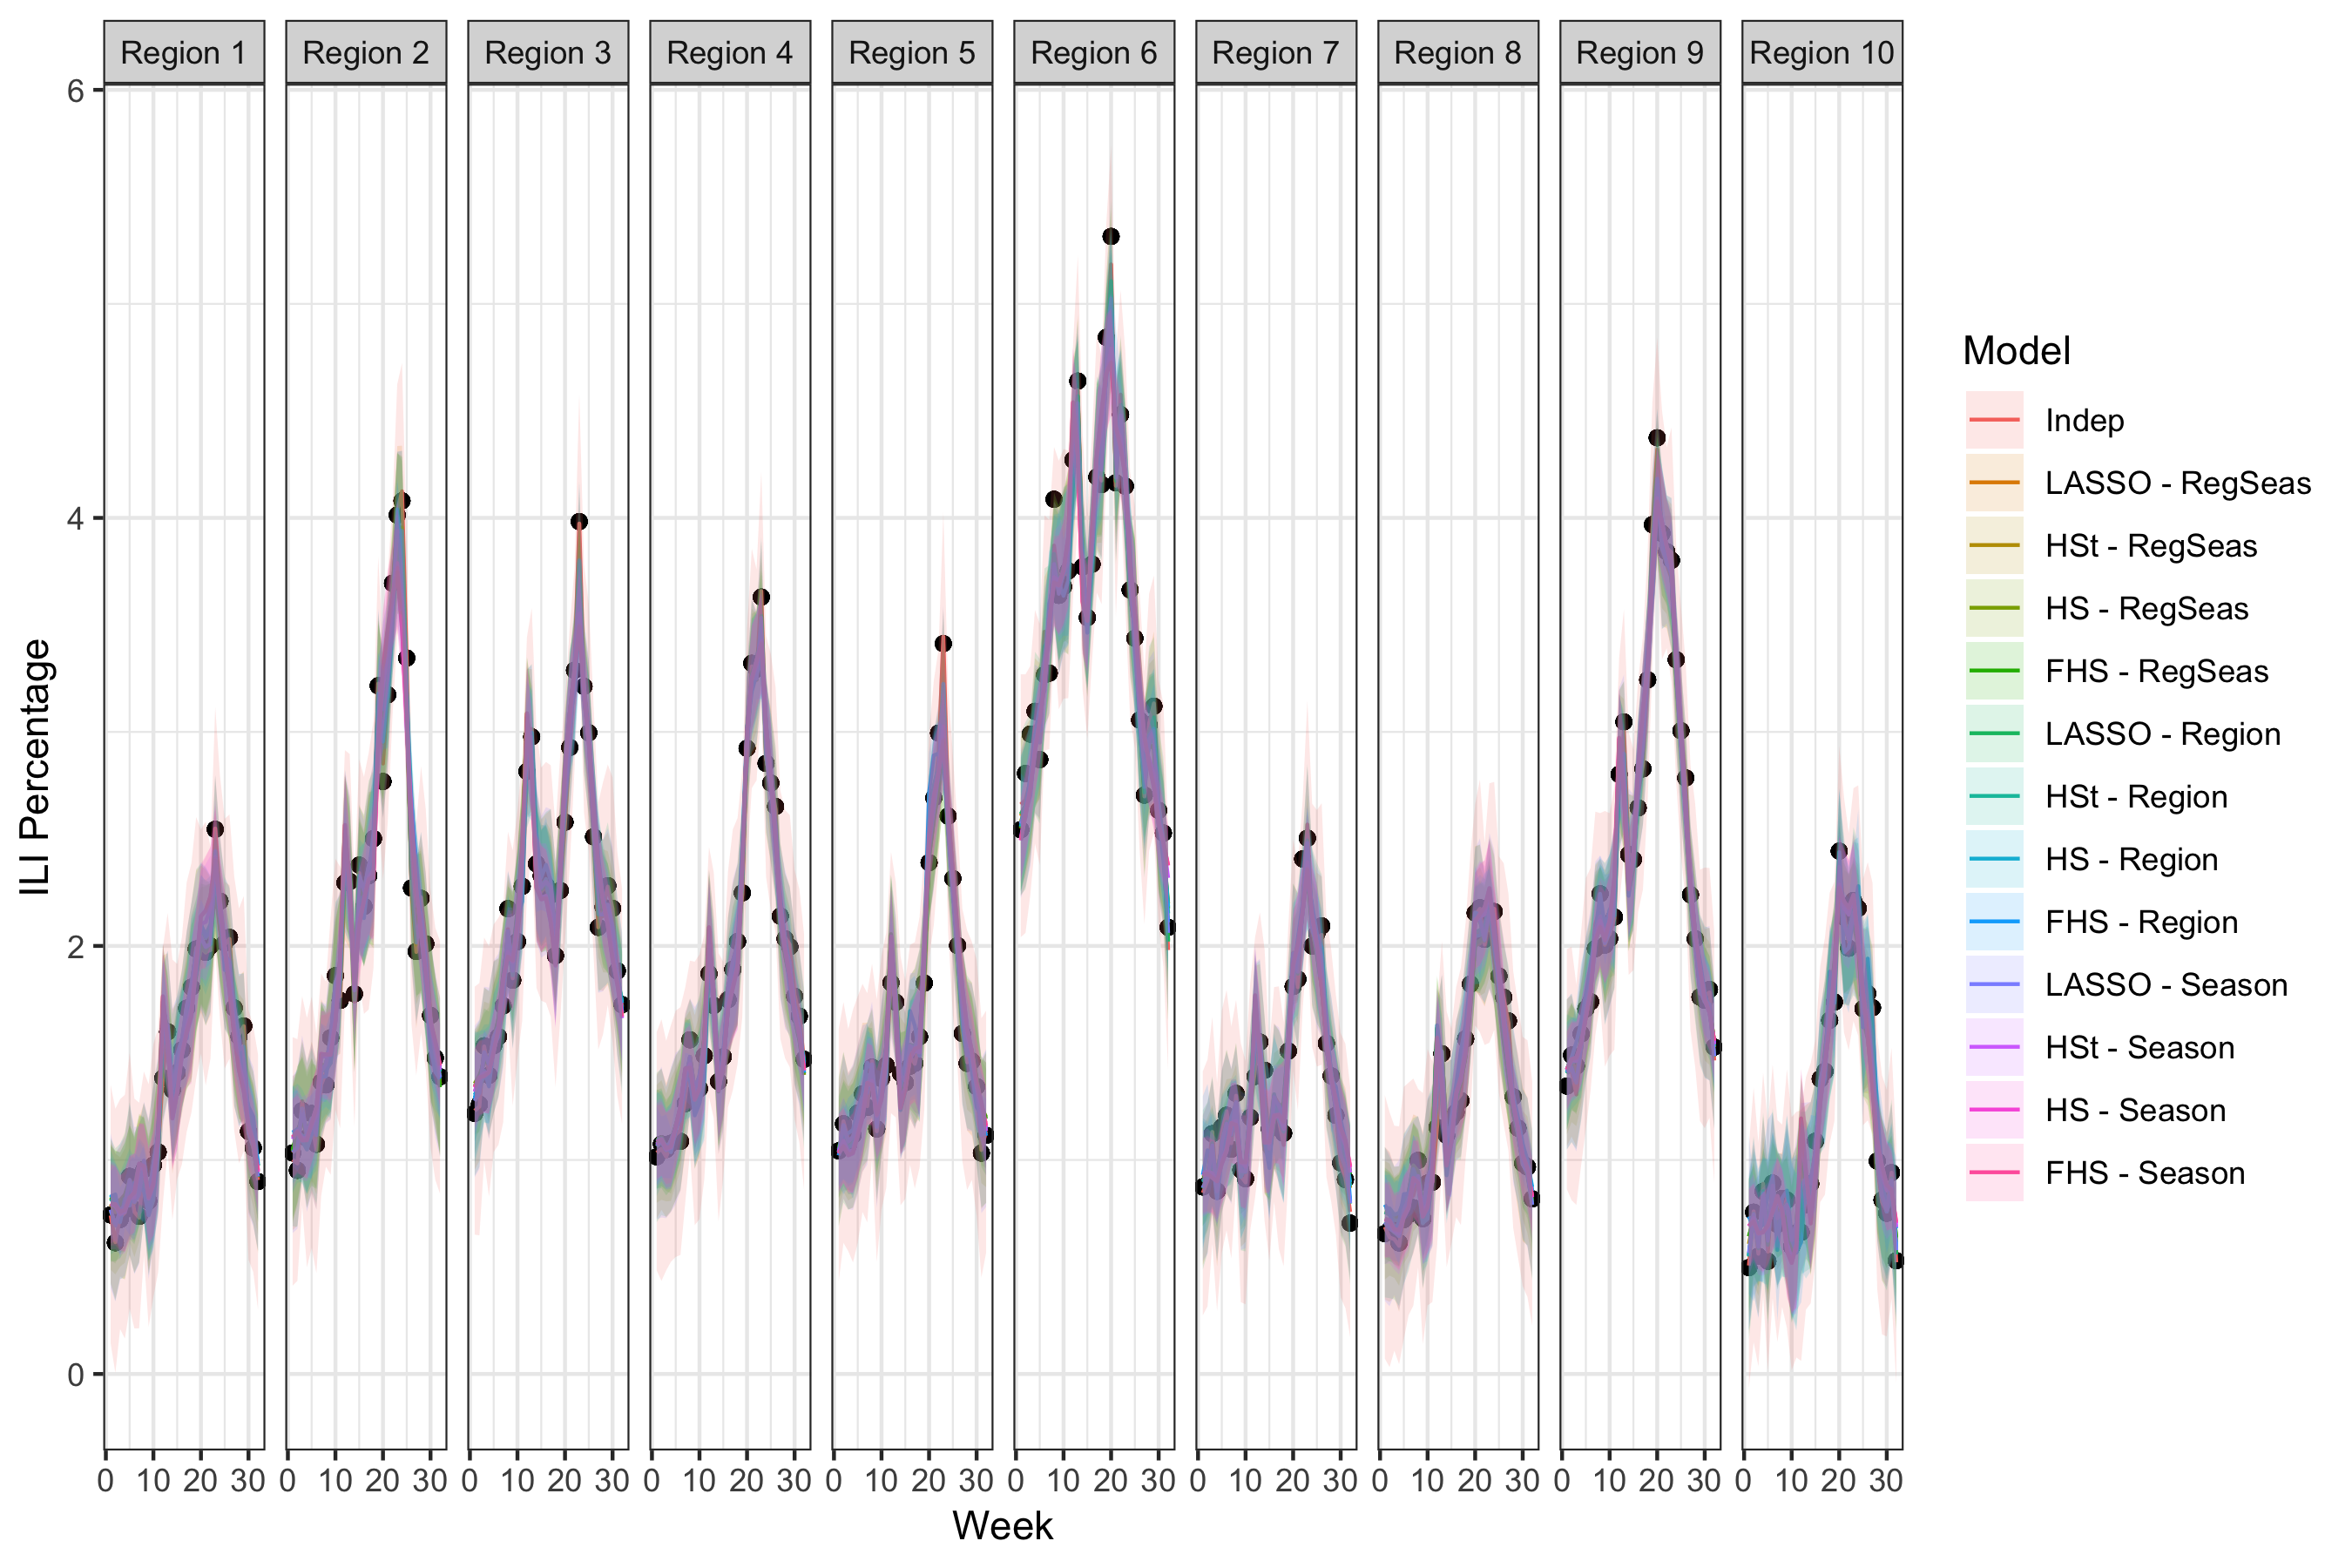
\includegraphics[width=0.8\linewidth]{plots/ILIfit.png}
% \caption{The 2015-2016 influenza season faceted by region.}
% \end{figure}
% 
% \end{block}

%----------------------------------------------------------------------------------------

\end{column} % End of column 2.1

\begin{column}{\onecolwid} % The second column within column 2 (column 2.2)

%----------------------------------------------------------------------------------------
%	PROOF OF VIETA'S FORMULAS
%----------------------------------------------------------------------------------------

% \begin{block}{$\text{M}_{eff}$}
% 
% \begin{figure}
% 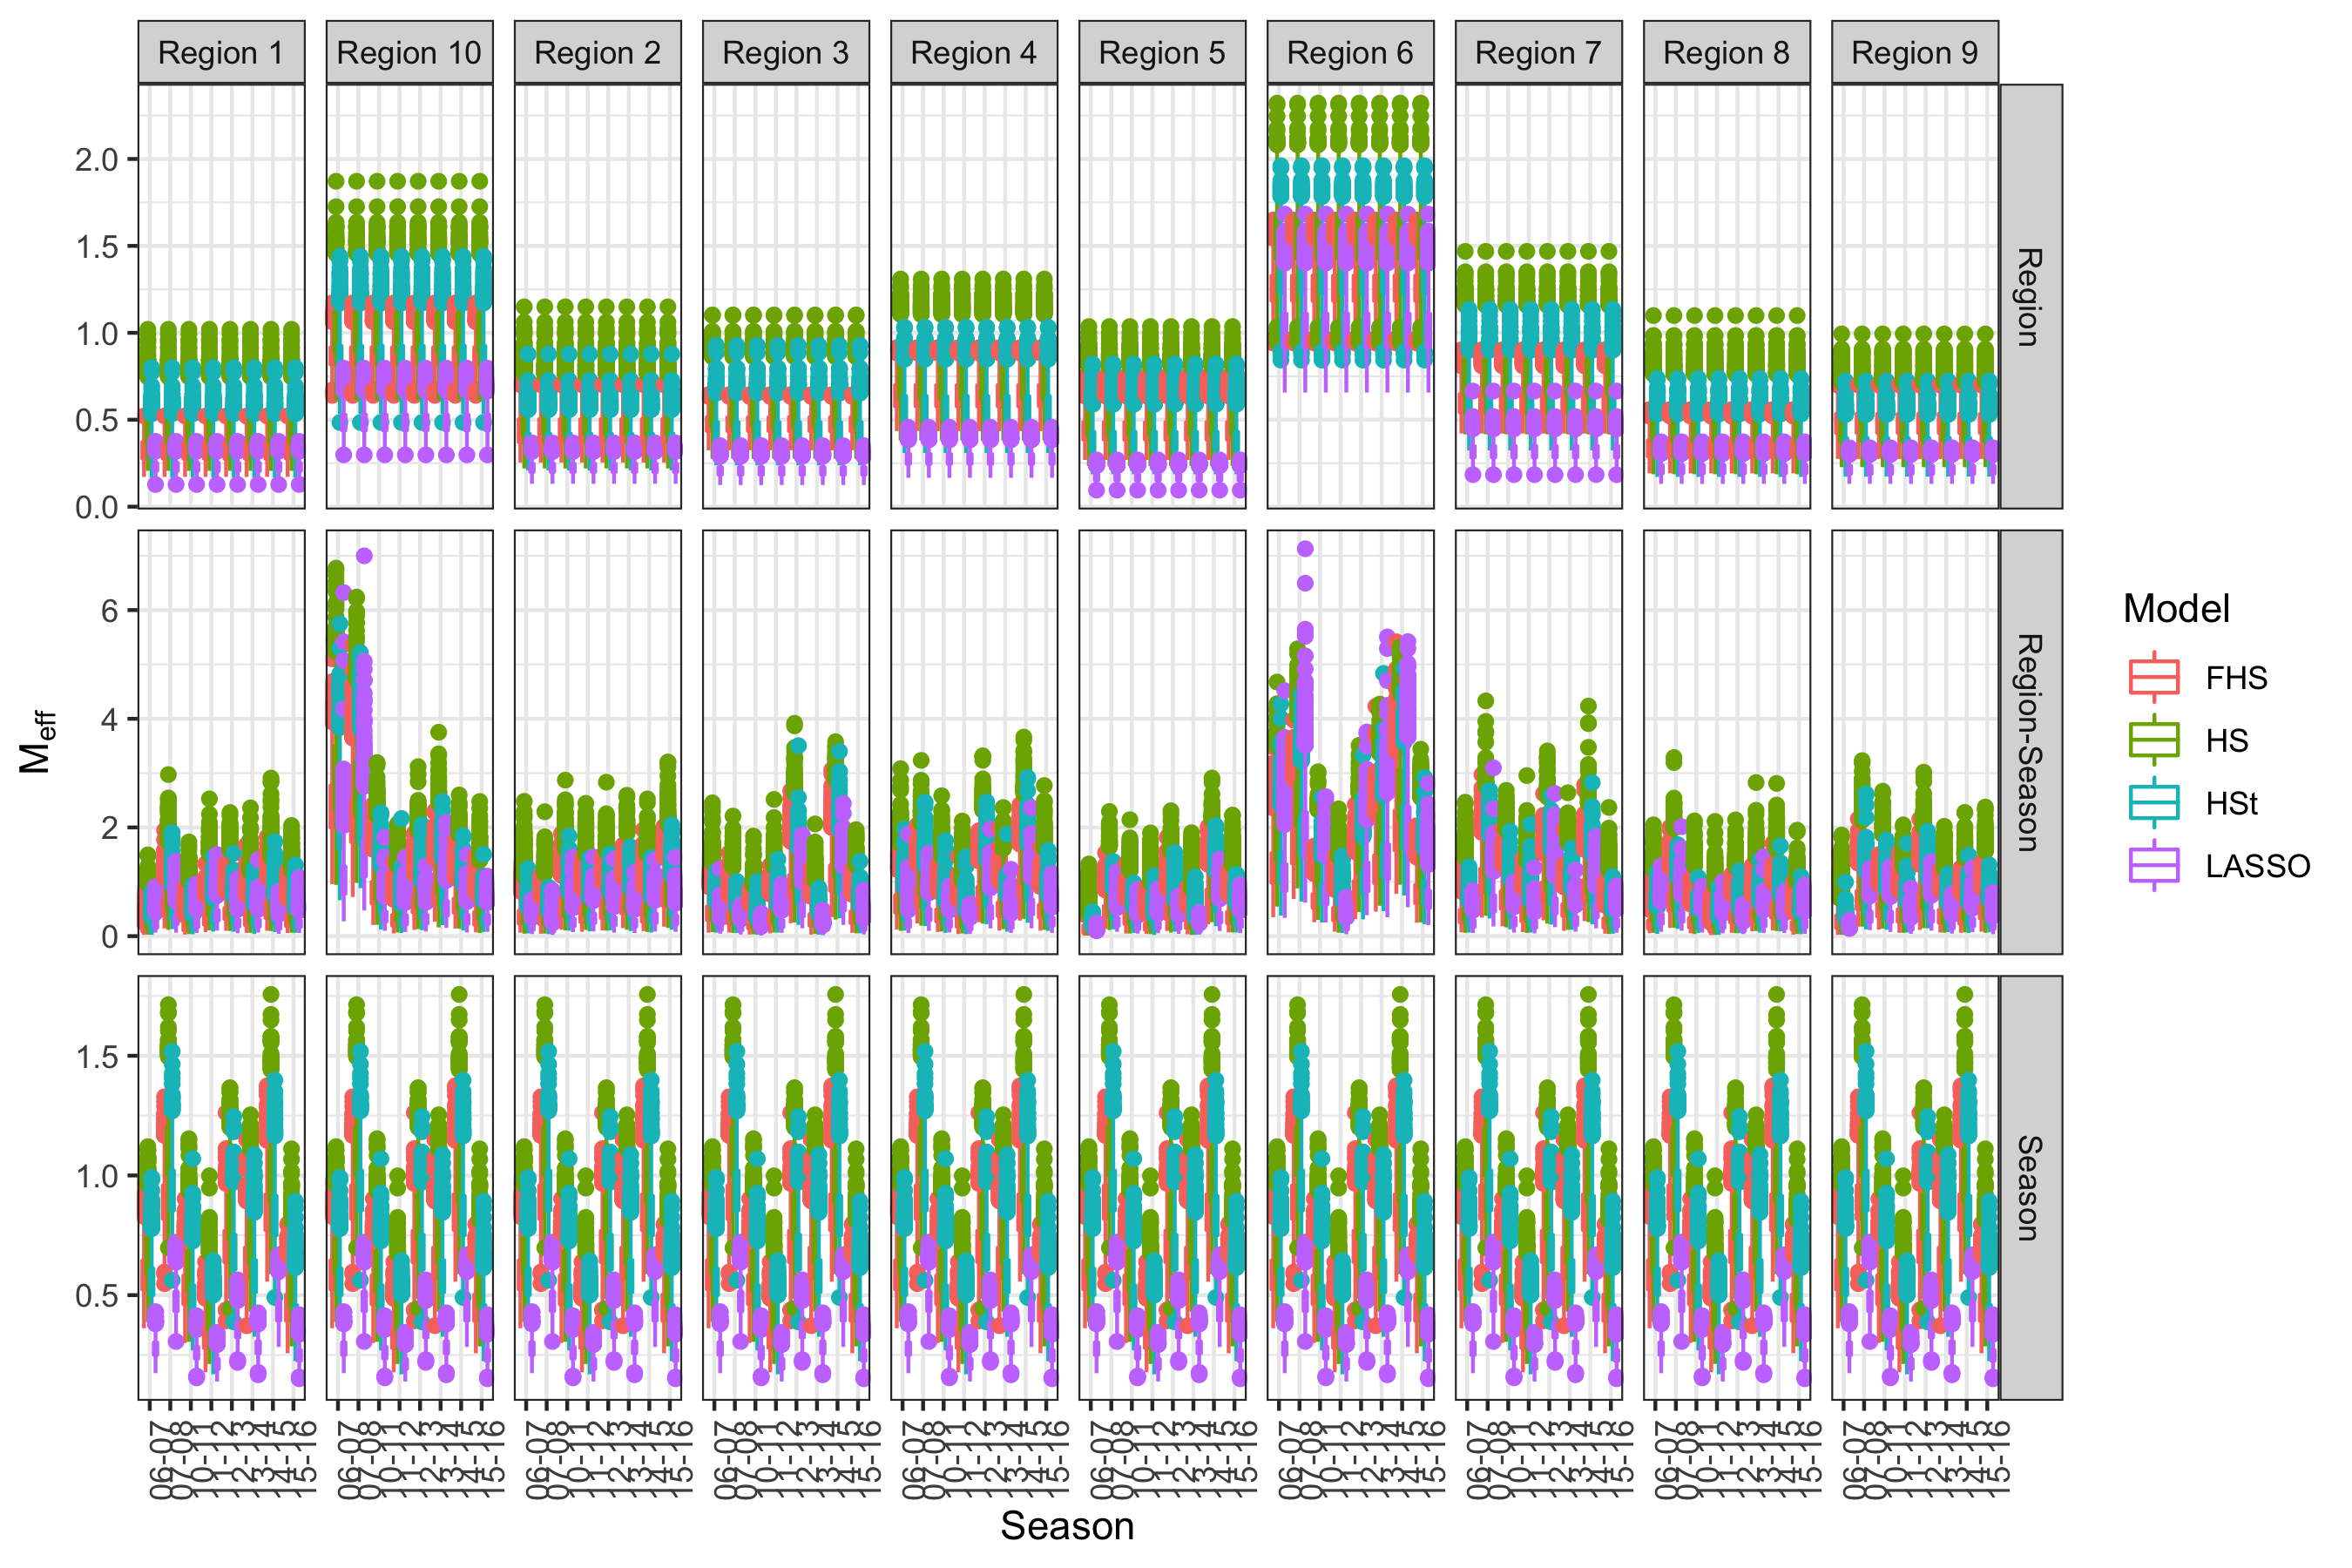
\includegraphics[width=0.8\linewidth]{plots/meff.png}
% \caption{The 2015-2016 influenza season faceted by region.}
% \end{figure}
% 
% \end{block}

%----------------------------------------------------------------------------------------

\end{column} % End of column 2.2

\end{columns} % End of the split of column 2

\end{column} % End of the second column

\begin{column}{\sepwid}\end{column} % Empty spacer column

\begin{column}{\onecolwid} % The third column

%----------------------------------------------------------------------------------------
%	CONCLUSION
%----------------------------------------------------------------------------------------

\begin{block}{Basis Selection}

\begin{figure}
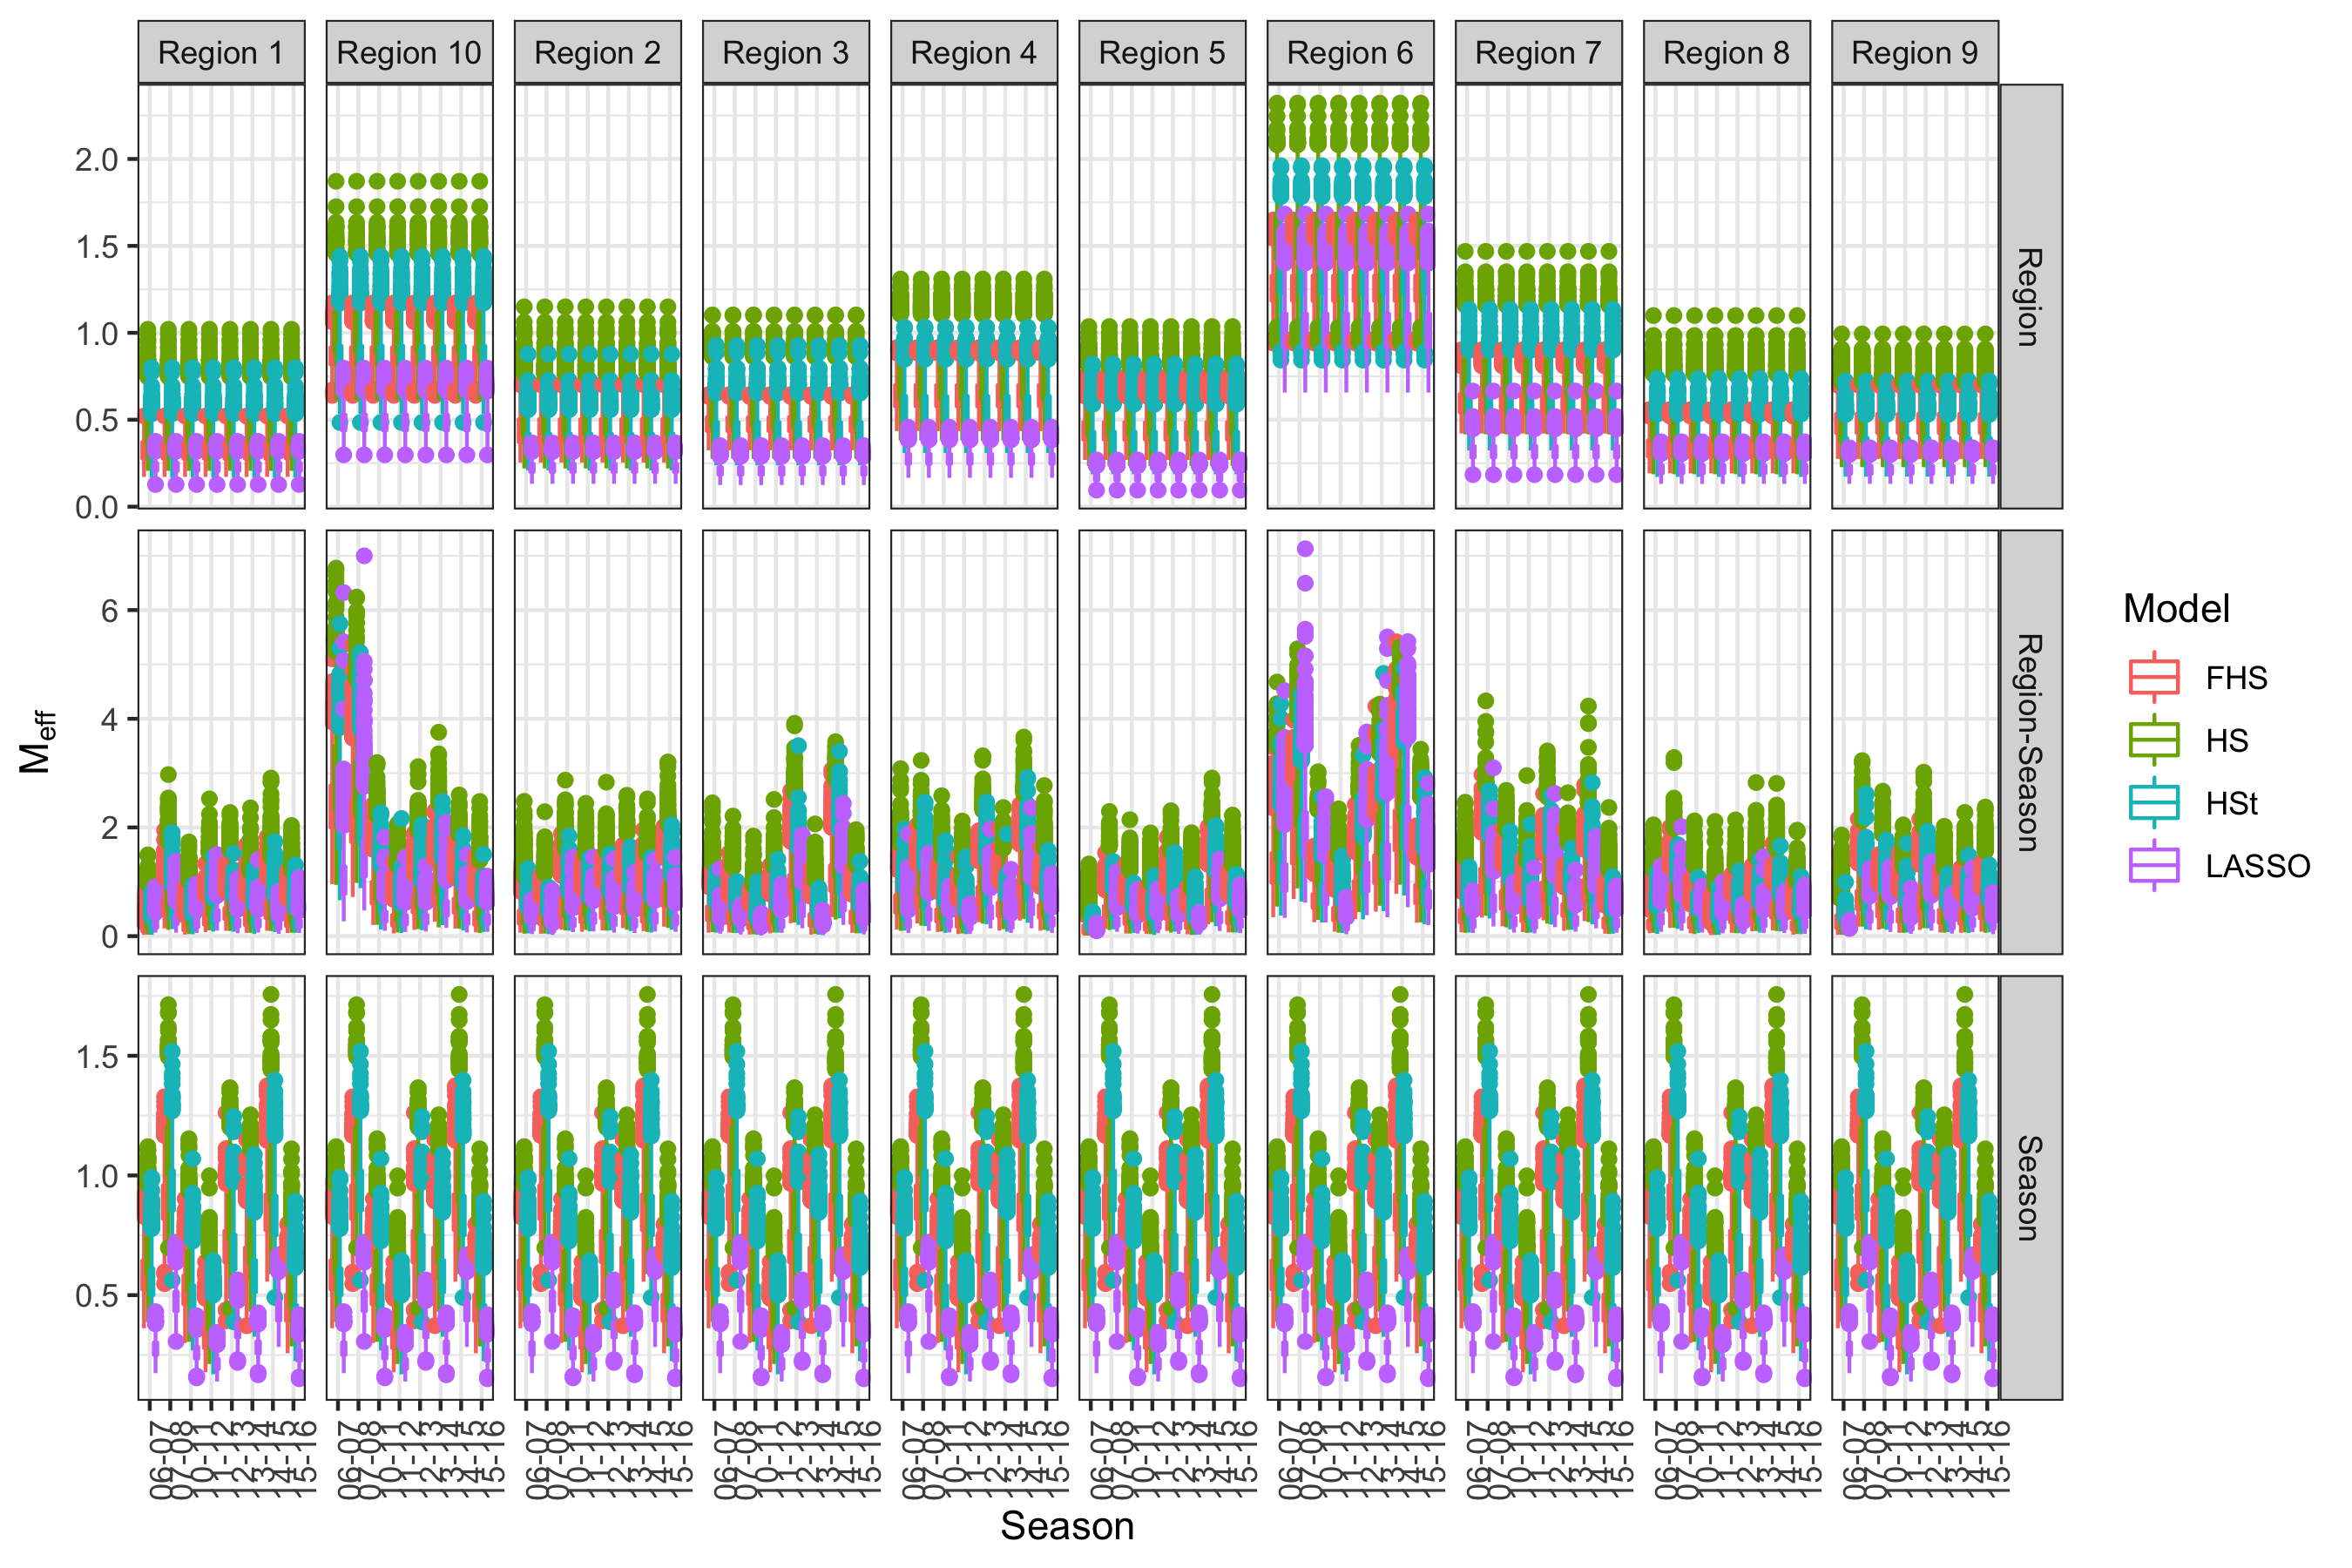
\includegraphics[width=\linewidth]{plots/meff.png}
\caption{$\text{M}_{eff}$ for the model fits.}
\end{figure}

% \begin{figure}
% 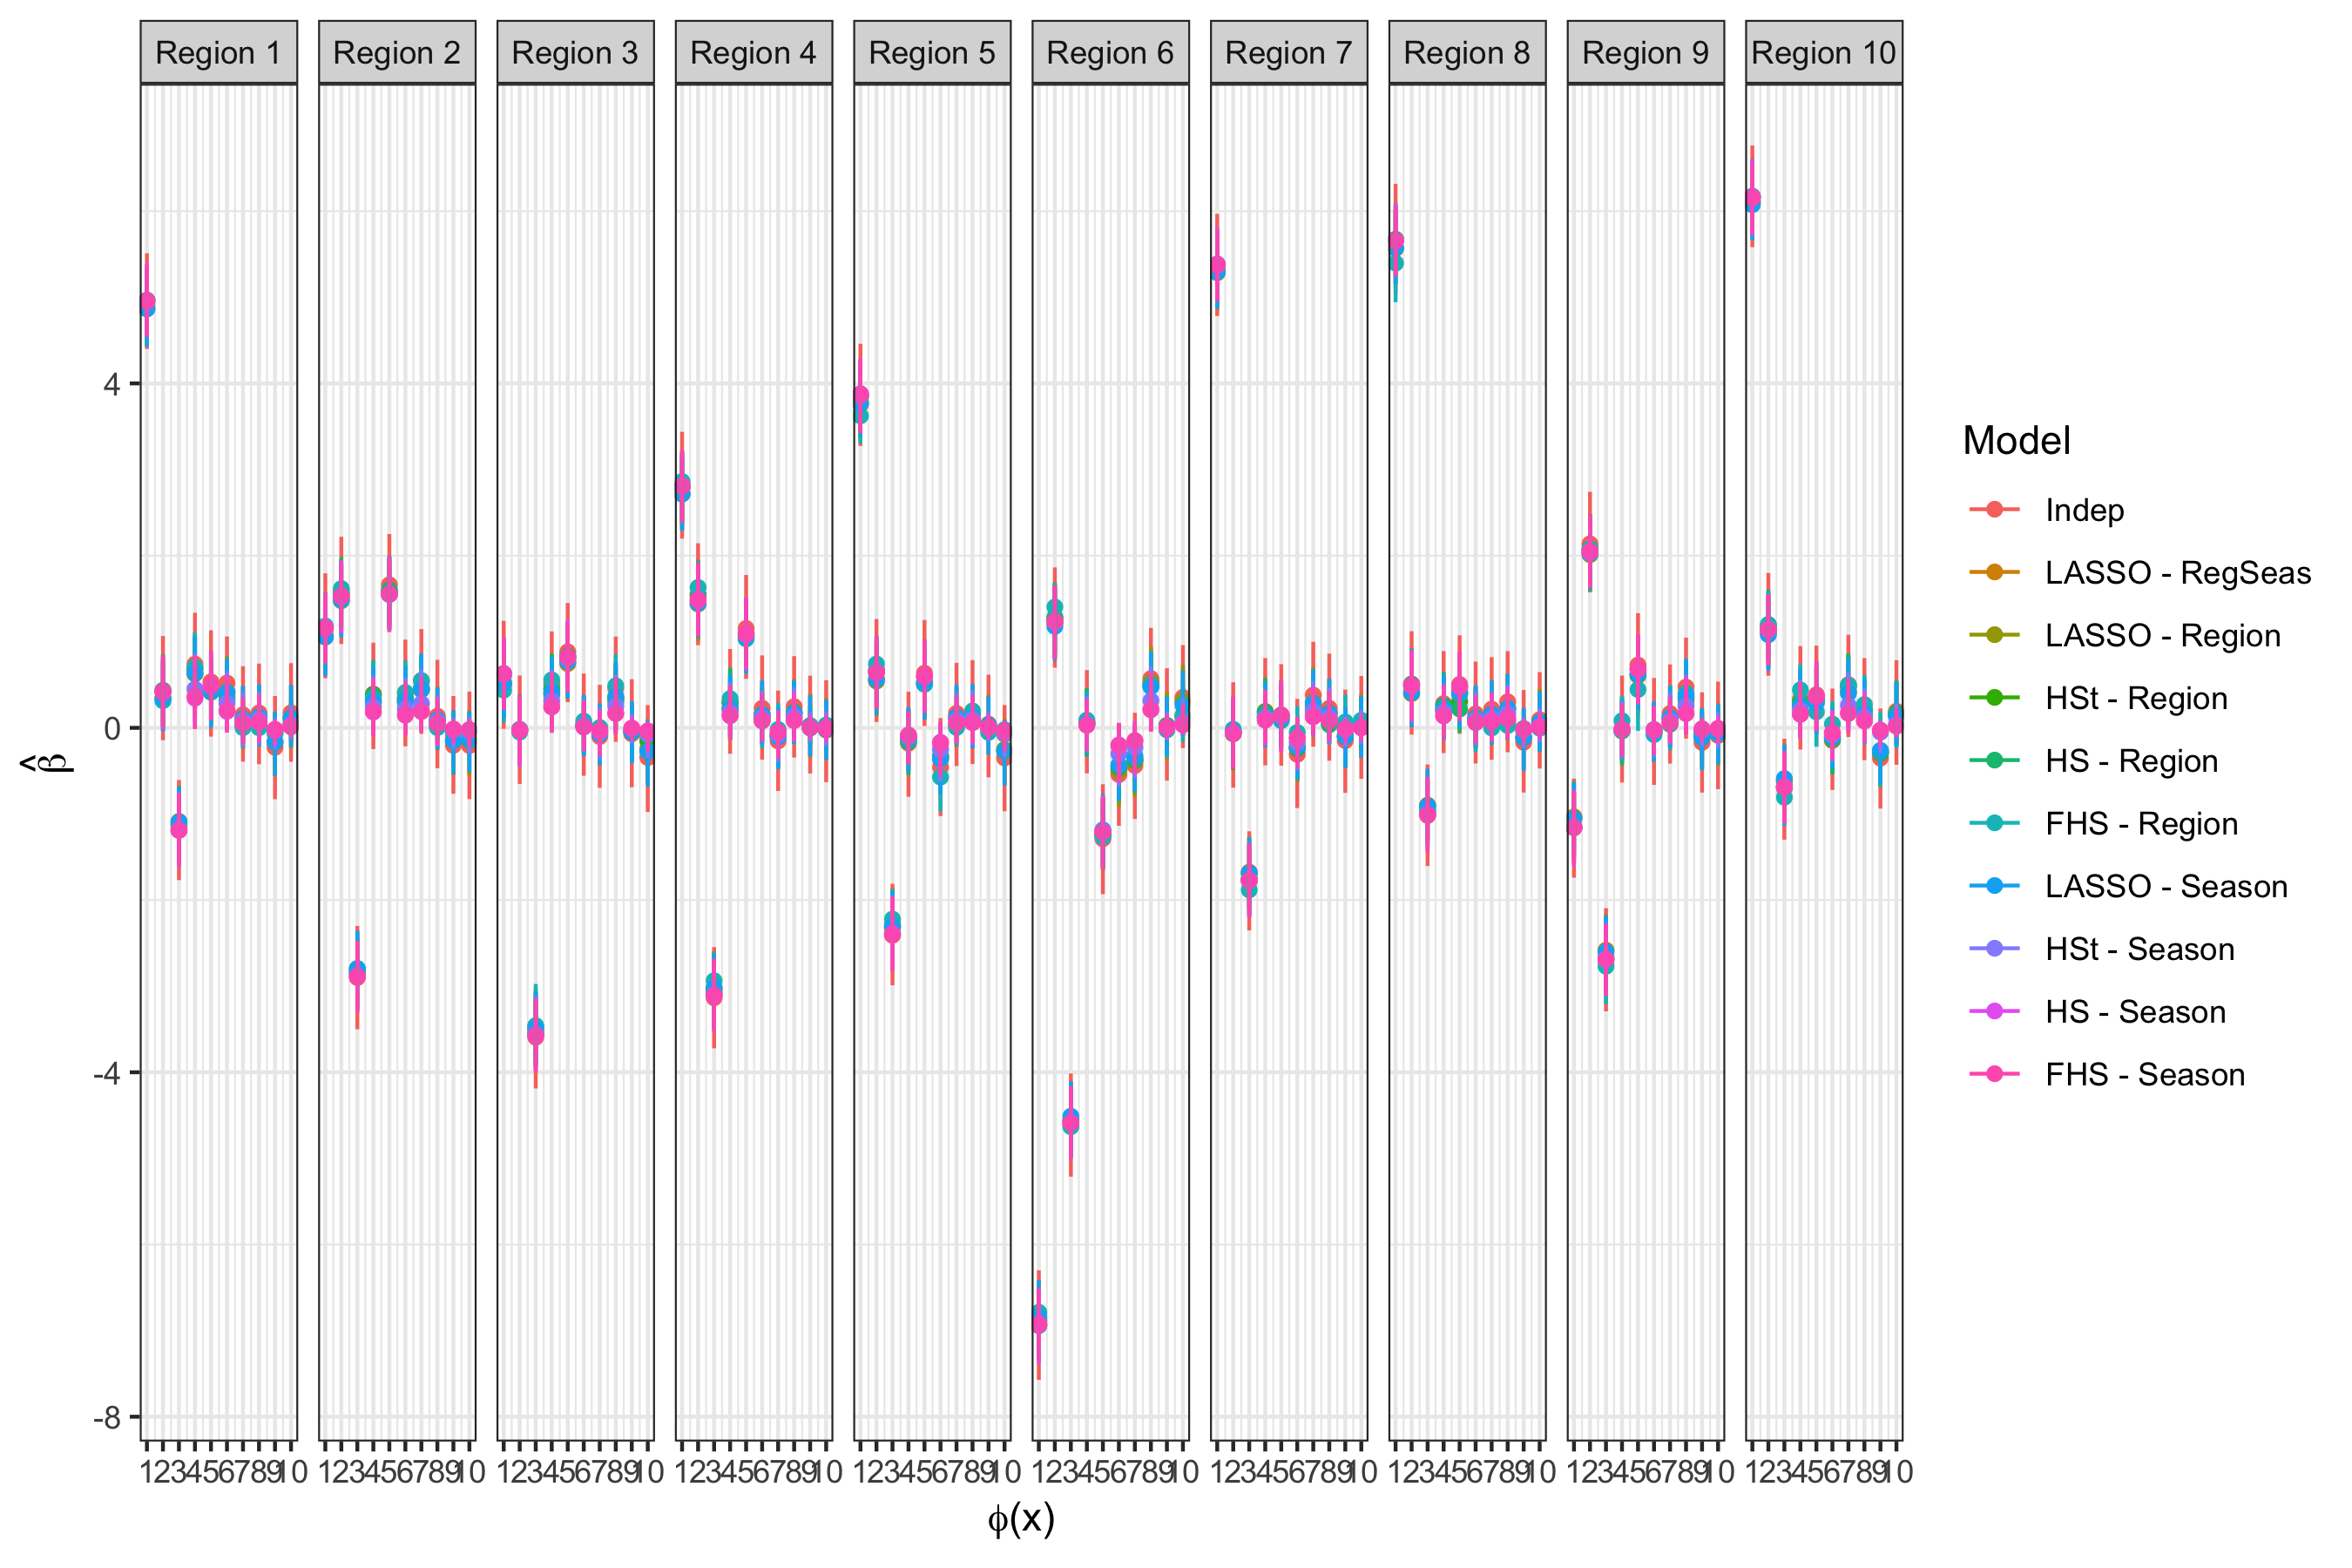
\includegraphics[width=\linewidth]{plots/beta_sing_seas.png}
% \caption{$\beta$ estimates and their $95\%$ credible intervals.}
% \end{figure}

\end{block}

\vspace{-20mm}

\begin{block}{Forecasting}
\begin{figure}
\includegraphics[width=\linewidth]{../../thesis/Chapter2/figures_tables/fc10.png}
\caption{This plot shows the $\beta$ estimates for the forecasted season across all regions.}
\end{figure}
\end{block}

\vspace{-20mm}

%----------------------------------------------------------------------------------------
%	ACKNOWLEDGEMENTS
%----------------------------------------------------------------------------------------

\begin{block}{Conclusions}

\begin{itemize}
\item Bayesian FPCA provides a flexible framework \\
\item Sprinkage priors allow the data to speak and chose min. basis\\
\item Hierarchy structures are good \\
\item Forecasting results are good \\
\end{itemize}

\end{block}

% \vspace{-10mm}

\begin{block}{References}

\setbeamertemplate{bibliography item}[text]
\nocite{*}
\bibliographystyle{siam}
\bibliography{poster}

\end{block}



%----------------------------------------------------------------------------------------

\end{column} % End of the third column

\end{columns} % End of all the columns in the poster

\end{frame} % End of the enclosing frame

\end{document}